\chapter{Diseño e implementación} % Main chapter title
\label{Chapter3} % Change X to a consecutive number; for referencing this chapter elsewhere, use \ref{ChapterX}

En este capítulo se comienza describiendo el flujo de trabajo utilizado, explicando la diferencia entre los ambientes locales y dockerizados. Luego, se describe la arquitectura de cada uno de estos ambientes. Después, se detallan los pasos realizados para preprocesar datos, como así también para entrenar y optimizar los hiperparámetros de los modelos. Posteriormente, se explica cómo se configuran el \textit{tracking server} y Airflow. Finalmente, se describe el diseño del servicio web que permite realizar predicciones.

\definecolor{mygreen}{rgb}{0,0.6,0}
\definecolor{mygray}{rgb}{0.5,0.5,0.5}
\definecolor{mymauve}{rgb}{0.58,0,0.82}

%----------------------------------------------------------------------------------------
%	SECTION 1
%----------------------------------------------------------------------------------------
\section{Flujo de trabajo}
\label{sec:flujo_trabajo}

En este trabajo se utilizó un flujo de trabajo que abarca desde la obtención de los datos base hasta la publicación de un servicio web, y  puede ser resumido en gran medida por la figura \ref{fig:flujo_trabajo}.

\begin{figure}[htbp]
	\centering
	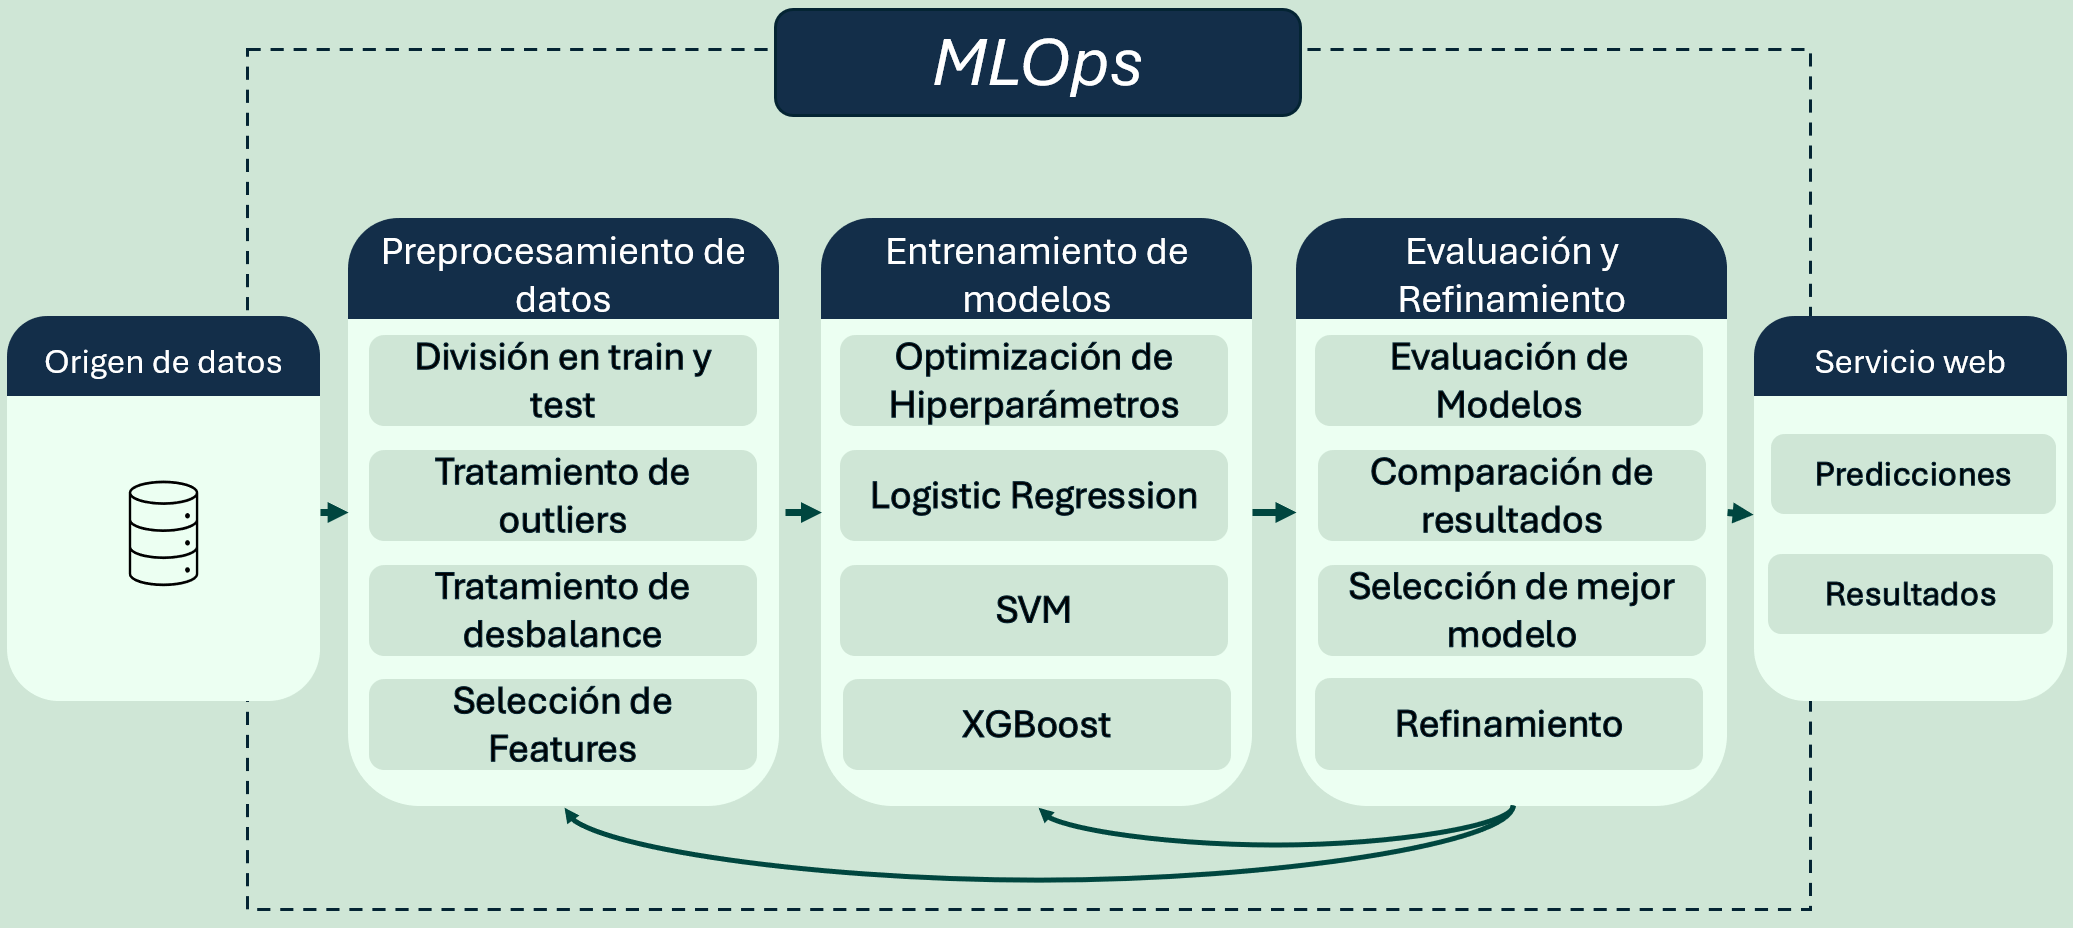
\includegraphics[width=0.9\textwidth]{./Figures/diagramaEnBloques.png}
	\caption{Flujo de trabajo utilizado.}
	\label{fig:flujo_trabajo}
\end{figure}

\subsection{Etapas del flujo de trabajo}

La primera etapa del flujo de trabajo implementado consta de la obtención del origen de datos del sistema: el dataset de \textit{Taiwanese Bankruptcy Prediction} \citep{taiwanese_bankruptcy_prediction_572}. Este es de origen público y cuenta con más de 6800 registros, que tienen información financiera de empresas del mercado de Taiwán entre 1999 y 2009.
La última etapa consiste en la publicación de un servicio web, que permitirá a los distintos usuarios realizar predicciones utilizando un modelo entrenado en este trabajo.

Entre estas dos etapas se encuentran otras que se caracterizan por ejecutarse de manera iterativa. Esto se debe a que se busca mejorar los resultados de las iteraciones anteriores, ya sea modificando algunos de sus parámetros o alterando la cantidad y/o el orden de sub-tareas dentro de cada etapa. Estas son:

\begin{itemize}
    \item Preprocesamiento de datos: en que, a grandes razgos, se mejora la calidad de dataset. Entre sus sub-tareas se encuentran la división del dataset en train y test, tratamiento de \textit{outliers}, tratamiento de desbalance y selección de \textit{features}.
    \item Entrenamiento de modelos: en que se crean, entrenan y optimizan modelos de \textit{machine learning}, utilizados para realizar predicciones de quiebra.
    \item Evaluación y refinamiento de modelos: en que se evalúan los modelos de la etapa anterior y se selecciona al mejor de ellos.
\end{itemize}

\subsection{Implementación del flujo de trabajo}

Para implementar el flujo de trabajo se optó por definir dos ambientes: un ambiente local y otro dockerizado.

El ambiente local se utiliza principalmente para experimentar distintas técnicas, herramientas e incluso sus posibles combinaciones. Por este motivo, este ambiente está constituído por \textit{notebooks} de python. Una vez determinada cuáles son las mejores técnicas y en qué orden deben ejecutarse, se procede a replicarlas en el ambiente dockerizado.

Por su parte, el ambiente dockerizado está orientado a la automatización del flujo de trabajo. De ahí a que se utilicen distintos contenedores de docker. Estos se crean para las etapas desde la descarga del dataset hasta la exposición de los modelos mediante un servicio web.

%----------------------------------------------------------------------------------------
%	SECTION 2
%----------------------------------------------------------------------------------------
\section{Arquitectura del sistema}

En la sección \ref{sec:flujo_trabajo} se describe el porqué del uso de dos ambientes al implementar el flujo de trabajo. En esta sección se describe la arquitectura de cada uno de estos ambientes. Igualmente, se remarca que en las futuras secciones y capítulos, al hablar de "sistema"\ se hará referencia al sistema desplegado mediante el ambiente dockerizado.

\subsection{Arquitectura del ambiente local}

El ambiente local se caracteriza por estar compuesto por un total de cinco directorios, cada uno dedicado a explorar distintas técnicas y/o herramientas. Cada directorio tiene una cantidad distintas de notebooks de python, que se ejecutan en el orden indicado en la figura \ref{fig:flujo_trabajo_local}. Por su parte, las notebooks generan dos datasets, uno para los datos de entrenamiento o \textit{train}, y otro para los datos de pruebas o \textit{test}. Estos datasets son a su vez utilizados como inputs por las notebooks del directorio siguiente en la secuencia de ejecución.

\begin{figure}[htbp]
	\centering
	
\includegraphics[width=0.95\textwidth]{./Figures/diagrama_componentes_local.png}
	\caption{Arquitectura del ambiente local.}
	\label{fig:flujo_trabajo_local}
\end{figure}

El primer directorio que se tiene en el ambiente local es el de análisis exploratorio. Éste, mediante la única notebook presente, se encarga de descargar el dataset original con el fin de analizarlo. En esta notebook se exploran las \textit{features} del dataset y su columna \textit{target} del dataset, haciendo foco en sus distribuciones, búsqueda de valores nulos y atípicos, como así también en la cantidad de clases presentes en la columna \textit{target}. Como esta es una notebook con fines exploratorios, el dataset de salida es el mismo que el de entrada.

El segundo directorio también consta de una sola notebook. Su objetivo es el de dividir al dataset original en un dataset de \textit{train} y otro de \textit{test}. Estos datasets nuevos constituyen la salida de este directorio, y son utilizados como entrada del siguiente.

El tercer directorio consta de dos notebooks: una para procesar datos nulos y otro para procesar \textit{outliers}. Como los datasets no tienen nulos, los datasets de salida quedan definidos por el notebook de procesamiento de \textit{outliers}.

El cuarto directorio está orientado al \textit{feature engineering}. En este se ejecutan las notebooks de escalado de datos, balanceo de datasets y selección de features de manera secuencial, generando un nuevo dataset de \textit{train} y \textit{test}.

Finalmente, en el quinto directorio se tienen tres notebooks que se ejecutan individualmente. Estas se encargan de optimizar los hiperparámetros y entrenar a los tres modelos de \textit{machine learning} utilizados en este trabajo. Finalmente, cada notebook genera un modelo distinto como salida, que se utilizan localmente para obtener métricas. A partir de estas métricas es que se decide si la ejecución total de notebooks es buena o no, y en caso de serlo, será replicada en el ambiente dockerizado.

\subsection{Arquitectura del ambiente dockerizado}

El ambiente dockerizado consta de cinco módulos principales, entre los que se encuentra el servicio web con el que los usuarios y/o interesados pueden interactuar, ya sea solicitando realizar predicciones o consultando métricas y/o gráficos. En la figura \ref{fig:flujo_trabajo_dockerizado} se puede esta arquitectura.

\begin{figure}[htbp]
	\centering
	
\includegraphics[width=0.95\textwidth]{./Figures/diagrama_componentes.png}
	\caption{Arquitectura del ambiente dockerizado.}
	\label{fig:flujo_trabajo_dockerizado}
\end{figure}

En el primer módulo se realiza la descarga del dataset, la división de \textit{train} y \textit{test}, y el preprocesamiento. Es decir, este módulo abarca las tareas realizadas en los primeros tres directorios del ambiente local.

En el segundo módulo se realiza la optimización de hiperparámetros y el entrenamiento de los modelos de \textit{machine learning}. Si bien estas dos tareas son secuenciales, las ejecuciones correspondientes a cada modelo se realizan en paralelo. Como salida se obtienen los tres modelos, que son utilizados por los módulos de \textit{tracking server} y "mejor modelo".

El módulo de "mejor modelo", como su nombre lo indica, se encarga de comparar los modelos de \textit{logistic regression}, SVM y XGBoost en función de sus métricas. A partir de esto es que se decide cuál de ellos es el mejor. Este modelo será guardado en el \textit{tracking server}, para que posteriormente puede ser utilizado por el servicio web para realizar predicciones.

El \textit{tracking server} consiste en una implementación de MLFlow. Mediante este, se tiene un servidor en donde se almacenan todas las versiones de los modelos entrenados, sus métricas, sus gráficos, como así también todas las versiones del mejor modelo. De esta manera, se puede acceder a esta información en cualquier momento.

Uno de los componentes que accede al \textit{tracking server} es el servicio web. Más precisamente, accede a la última versión del mejor modelo. También accede a las métricas y gráficos de la última versión de cada modelo entrenado. Esto le permite responder a las solicitudes de usuarios, ya sea para realizar inferencias, como también para responder consultas respecto a métricas y/o gráficas.

%----------------------------------------------------------------------------------------
%	SECTION 3
%----------------------------------------------------------------------------------------
\section{Preprocesamiento de datos}
\label{sec:preprocesamiento_de_datos}

El preprocesamiento abarca las tareas relacionadas a la división de dataset, tratamiento de nulos y de \textit{outliers}, escalado de datos, balanceo de dataset y selección de \textit{features}. A continuación se detalla en que consiste cada una de estas tareas.

\subsection{División del dataset}
\label{subsec:division_dataset}

El dataset original de \textit{Taiwanese Bankruptcy Prediction} \citep{taiwanese_bankruptcy_prediction_572} cuenta con un total de 6819 registros, entre los que hay un total de 220 casos de empresas que entran en quiebra. Si bien estos datos son suficientes para entrenar los modelos de \textit{machine learning} deseados, se presentan dos inconvenientes.

El primero es que hay un desbalance del dataset, siendo la clase objetivo mayoritaria la de empresas que no entran en quiebra. El segundo problema consiste en la necesidad de datos para evaluar qué tan bien generalizan los modelos.

Mediante la división del dataset en \textit{train} o entrenamiento y \textit{test} o evaluación se podrá resolver parte de este problema. Esto permitirá tener un set de datos reservado exclusivamente para la evaluación de modelos. Para ello, se utilizará la función \texttt{train\_test\_split} \citep{WEBSITE:train_test_split} de la biblioteca \texttt{scikit-learn} \citep{WEBSITE:scikit-learn}. Esta función además cuenta con el parámetro \texttt{stratify}, que permite dividir una clase en particular proporcionalmente entre los datasets resultantes.

Al implementar la función \texttt{train\_test\_split} se opta por generar un dataset de \textit{test} equivalente al 30\% de los datos originales, es decir, 2046 registros de un total de 6819. A su vez, mediante el parámetro \texttt{stratify}, se logra una distribución proporcional de registros de empresas en quiebra, quedando 154 para \textit{train} y 66 para \textit{test}.

\subsection{Tratamiento de nulos y outliers}

En este caso comienza buscando la presencia de datos nulos en los datasets de \textit{train} y \textit{test}. Al analizar todas las columnas de estos dataset, no se encontraron nulos, por lo que tampoco se aplican medidas de corrección.

En cuanto a los \textit{outliers} o datos atípicos, se utiliza la técnica rango intercuartil o IQR para detectarlos. Para tratarlos, se implementan las técnicas de imputación por media, imputación por mediana, imputación por moda, transformación por raíz cuadrada y transformación de Yeo-Johnson. Todas estas técnicas son explicadas en las sección \ref{subsec:tecnicas_procesamiento}.

Los cálculos del IQR y de las medidas de tendencia central (media, moda y mediana) se hicieron sobre el dataset de \textit{train}, mas no sobre el de \textit{test}. Luego, en \textit{test} se consideran \textit{outliers} a aquellos valores que no se encuentren en el IQR de \textit{text}, según cada columna, y se imputan con los valores obtenidos en \textit{train}.

Esto es para evitar que haya \textit{data leakage}, es decir, que se filtren datos o características del dataset de \textit{test} en el dataset de \textit{train}. Si esto sucediese, los modelos de \textit{machine learning} entrenados con estos dataset con datos filtrados podrían aprender indirectamente algunas de estas características, lo que evitaría que generalicen correctamente. En cuanto a la transformación por raíz cuadrada y transformación de Yeo-Johnson, estas simplemente se aplican sobre todo el rango de valores de los datasets deseados por separado.

Para definir qué técnica se aplica en cada columna, se opta por primero aplicar las cinco técnicas a cada columna. Luego, para cada técnicas, se calculan cuántos \textit{outliers} hay en la columna modificada. Finalmente, se elige a aquella técnica que haya generado la menor cantidad posible de \textit{outliers}.

Si bien este método ayuda a reducir la cantidad de datos atípicos, estos no serán siempre cero. Por ejemplo, la variable \texttt{total asset turnover} se trató con la transformación de Yeo-Johnson, que redujo los \textit{outliers} de 247 a cero, tal como se ve en la figura \ref{fig:transformacion-yeo-johnson}.

\begin{figure}[htbp]
	\centering
	
\includegraphics[width=0.95\textwidth]{./Figures/transformacion-yeo-johnson.png}
	\caption{Transformación de Yeo-Johnson sobre la columna \texttt{Total Asset Turnover}.}
	\label{fig:transformacion-yeo-johnson}
\end{figure}

Pero, para el caso de la variable \texttt{cash flow per share}, la técnica que menos \textit{outliers} genera es la de imputación por mediana, tal como se ve en la figura \ref{fig:imputacion-por-mediana}, la que reduce los \textit{outliers} de 383 a 191.

\begin{figure}[H]
	\centering
	
\includegraphics[width=0.95\textwidth]{./Figures/imputacion-por-mediana.png}
	\caption{Imputación por mediana sobre la columna \texttt{Cash Flow Per Share}.}
	\label{fig:imputacion-por-mediana}
\end{figure}

\subsection{Escalado de datos}

Las distintas columnas de los datasets presentan diferentes rangos de valores. Esto es un factor que puede perjudicar a los modelos entrenados con dichos datos, ya que pueden priorizar erróneamente una columna frente a otras solamente por esta diferencia de rangos. Por ello, es fundamental escalar los datos antes de entrenar ciertos modelos de \textit{machine learning}.

Para el escalado de datos se toma una estrategia similar a la del tratamiento de \textit{outliers}: las técnicas de escalado se ajustan en el dataset de \textit{train}, y se aplican en ambos datasets. De esta manera se evita el \textit{data leakage} en esta etapa.

En este caso solo se estudia e implementa la técnica de StandardScaler \citep{WEBSITE:standardscaler}. El beneficio se encuentra al entrenar modelos de \textit{logistic regression} y SVM, ya que permite mejorar sus reultados. Por su parte, el modelo XGBoost es más robusto a la diferencia de escalas entre columnas. Esto se puede observar en el paper de \textit{The Impact of Feature Scaling In Machine Learning: Effects on Regression and Classification Tasks} \citep{article:feature-scaling}.

El efecto se puede observar, por ejemplo, en los casos de las columnas \texttt{total expense/assets} y \texttt{retained earnings to total assets} del dataset de \textit{train}. En la figura \ref{fig:standard-scaling-01}, en el histograma de la izquierda, se observa que la primera de estas columnas tiene un rango relativamente pequeño, que va desde el cero hasta el 0,03, con media de 0,02 y desvío de 0,01.

\begin{figure}[htbp]
	\centering
	
\includegraphics[width=0.95\textwidth]{./Figures/standard-scaling-caso-01.png}
	\caption{Standard scaler aplicado a \texttt{Total expense/assets}.}
	\label{fig:standard-scaling-01}
\end{figure}

Respecto a la columna \texttt{retained earnings to total assets}, en el histograma de la izquierda de la figura \ref{fig:standard-scaling-02}, se observa que el rango original es relativamente mayor, ya que va desde el 0,91 hasta el 0,96, con media 0,94 y desvío de 0,01. Al aplicar \textit{standard scaling} a ambas columnas (por separado) se observa que los rangos ahora se encuentran entre -3 y 3 (aproximadamente) para ambos casos, teniendo ambas una media de 0 y un desvío de 1.

\begin{figure}[htbp]
	\centering
	
\includegraphics[width=0.95\textwidth]{./Figures/standard-scaling-caso-02.png}
	\caption{Standard scaler aplicado a \texttt{Retained Earnings to Total Assets}.}
	\label{fig:standard-scaling-02}
\end{figure}

\subsection{Balanceo del dataset}

Tal como se menciona en la sección \ref{subsec:division_dataset}, tanto el dataset original como los dataset resultantes al dividir en \textit{train} y \textit{test} presentan un desbalance en la columna objetivo \texttt{Bankrupt}, tal como se observa en la figura \ref{fig:descabalance-target}. Este tipo de problemas deben de resolverse antes de entrenar los modelos deseados, ya que, en caso contrario, los modelos podrían generalizar erróneamente nuevos casos.

\begin{figure}[htbp]
	\centering
	
\includegraphics[width=0.95\textwidth]{./Figures/desbalance.png}
	\caption{Desbalance de la columna Bankrupt? en el dataset de train.}
	\label{fig:descabalance-target}
\end{figure}

Para resolver el desbalance se realizan pruebas con SMOTE \citep{article:smote}, SMOTE-ENN \citep{article:smoteenn} y ADASYN \citep{article:adasyn}, técnicas que permiten generar datos sintéticos de distintas maneras, tal como se explica en la sección \ref{subsec:tecnicas_balanceo}. Como estos datos son sintéticos, las técnicas se aplican solamente en el dataset de \textit{train}, ya que aplicarlas a \textit{test} podría provocar \textit{data leakage}.

Los resultados de aplicar estas técnicas se observan en la tabla \ref{tab:resultados-balanceo}. En la misma se observa que SMOTE-ENN es la que menos registros generó, como así también la que mayor diferencia entre clases tiene (la clase positiva, o empresas que entran en quiebra, tiene 691 registros más que la otra clase). Igualmente, se opta por aplicar esta técnica en el flujo de trabajo final, ya que es la que mejor resutados arroja.

\begin{table}[H]
	\centering
	\caption[Técnicas utilizadas]{Resultados de las técnicas de balanceo de datos.}
	\begin{tabular}{c c c c c}
		\toprule
		\textbf{Técnica} 	 & \textbf{Registros nuevos} & \textbf{Clases positivas} & \textbf{Clases negativas}\\
		\midrule
        ADASYN & 9265 & 4646 & 4619 \\
        SMOTE & 9238 & 4619 & 4619  \\
        SMOTE-ENN & 8547 & 4619 & 3928 \\		
		\bottomrule
		\hline
	\end{tabular}
	\label{tab:resultados-balanceo}
\end{table}

\subsection{Selección de features}
\label{subsec:preproc_seleccion_features}

La última etapa del preprocesamiento consta de la selección de features. Mediante esta, se busca reducir la cantidad de columnas de los datasets, a modo de quedarse con aquellas que mayor información brindan sobre la columna objetivo.

Para este caso, solamente se implementa la técnica de información mutua, explicada en la sección \ref{subsec:seleccion_features}. En las primeras pruebas realizadas mediante esta técnica, se obtuvieron 66 columnas del dataset de \textit{train} que mejor explican a la variable \textit{target}. El resto de las columnas son posteriormente descartados en ambos datasets. Como el número 66 fue elegido al azar (más precisamente, se eligió al azar el 70\% de las columnas más representativas), se opta por configurar este valor representativo de la cantidad de columnas como un hiperparámetro al entrenar los distintos modelos. De esta manera, se obtiene el número que mejor resultados permita obtener en cuanto a predicciones.

Cabe aclarar que otra técnica estudiada es la de ANOVA \citep{article:anova}. Como prerequisito para aplicarla, es necesario que las distribuciones de cada columna sobre las categorías de la columna objetivo tengan distribución normal y sean homocedásticas (es decir, que tengan varianzas iguales). Como estos prerequisitos no se cumplen en el dataset de \textit{train}, se descartó el uso de la técnica de ANOVA para seleccionar features.

%----------------------------------------------------------------------------------------
%	SECTION 4
%----------------------------------------------------------------------------------------
\section{Optimización y entrenamiento de modelos}
\label{sec:optimizacion_y_training}

Una vez preprocesado el dataset original y generados los datasets de \textit{train} y \textit{test}, se comienza con el entrenamiento de modelos. A fin de generar los mejores modelos, se procede a optimizar sus hiperparámetros, como así también se realizan pruebas utilizando \textit{pipelines}.

\subsection{Pipelines y modelos}
\label{sec:pipelines_y_modelos}

En este trabajo se realizaron distintas pruebas con modelos de \textit{machine learning}. En todas estas, el preprocesamiento aplicado era el descrito en la sección \ref{sec:preprocesamiento_de_datos}, es decir, una serie de técnicas que, aplicadas sobre el dataset original, generaban un dataset final de \textit{train} y otro de \textit{test}. Luego, estos dataset se utilizan como \textit{input} de los modelos, tanto para entrenarlos como para evaluarlos. Pero ciertos modelos no presentaban buenos resultados. Un ejemplo es XGBoost, que en ciertas pruebas arroja un \textit{recall} de 0,42, un valor muy bajo.

Para mejorar esto, se utiliza la clase \texttt{Pipeline} \citep{WEBSITE:imblearn-pipeline} de \texttt{Imblearn} \citep{WEBSITE:imblearn}. Tal como su nombre lo indica, permite generar un \textit{pipeline} o secuencia de pasos sobre un dataset a fin de ajustarlo, y posteriormente transformar o aplicar los pasos tanto en este como en otros datasets. Las ventajas que poseen estos \textit{pipelines} es que procesan mejor los datos de datasets desbalanceados, manejan mejor el \textit{cross-validation} con \textit{resampling} (técnica que se explica posteriormente) y está específicamente diseñado para usarse al optimizar hiperparámetros.

A nivel implementación, el \textit{pipeline} utilizado consta de los mismos pasos definidos en el preprocesamiento: correción de datos atípicos, escalado, balanceo de datos y selección de features. Se agrega también un paso final correspondiente al entrenamiento del modelo, ya que mejoran los resultados tanto al entrenar como al optimizar hiperparámetros. Luego, mediante el método \texttt{fit} junto al dataset de \textit{train}, aplica las transformaciones a los datos y entrena al modelo, mientras que con el método \texttt{predict} junto al dataset de \textit{test} evalúa al modelo final.

En cuanto a resultados, la misma secuencia de transformaciones que se utilizaron para el modelo XGBoost y dieron un resultado para \textit{recall} de 0,42, con la implementación de la clase \texttt{Pipeline} dieron un \textit{recall} de 0,8. Por este motivo, se opta por utilizar \textit{pipelines} para entrenar y optimizar modelos.

\subsection{Cross validation e implementación durante optimización}

Con el fin de optimizar hiperparámetros se utiliza el \textit{framework} \texttt{optuna} \citep{article:optuna}. Este se caracteriza por utilizar optimización bayesiana \citep{artice:bayesion-optimization}, que permite determinar qué combinaciones de parámetros funcionarán mejor basándose en resultados anteriores, lo que permite ahorrar tiempo de cómputo.

Esta herramienta fue combinada con la técnica de \textit{cross validation}, que permite dividir el dataset en k subconjuntos o \textit{folds} iguales, con el fin de realizar k entrenamientos. Más precisamente, se utiliza un fold distinto para validar y el resto para entrenar. En particular, se utiliza la función \texttt{cross\_validate} \citep{WEBSITE:crossvalidate} de \texttt{scikit-learn} \citep{WEBSITE:scikit-learn}.

Este enfoque asegura que cada configuración de hiperparámetros sea evaluada de manera exhaustiva en diferentes subconjuntos de datos, lo que a su vez permite prevenir el \textit{overfitting} y mitigar el \textit{data leakage}. También permite obtener una estimación robusta del entrenamiento, ya que se promedian los resultados de los k experimentos.

En este trabajo se opta por utilizar 5 folds, entrenados durante 100 iteraciones de \texttt{optuna}. Esto se implementa mediante la clase \texttt{StratifiedKFold} \citep{WEBSITE:stratifiedkfold}, que mediante el parámetro \texttt{shuffle} permite mezclar los datos para evitar sesgos.

Otra herramienta utilizada es \texttt{MedianPruner} \citep{WEBSITE:MedianPruner}, que permite realizar una exploración más profunda del espacio de búsqueda en menor tiempo. Esto lo logra al detener automáticamente los ensayos cuyos resultados preliminares, es decir, durante los primeros folds de la validación cruzada, no superan la mediana de rendimiento de intentos anteriores.

Finalmente, a la hora de optimizar mediante \texttt{optuna}, se busca maximizar la métrica de AUPRC. Esta métrica es ideal ya que, tal como se menciona en el paper \textit{A closer look at AUROC and AUPRC under class imbalance} \citep{article:closer_look_auprc}, es ideal para utilizar en casos en que existe desbalanceo de clases. En particular, esta métrica se obtiene al configurar el parámetro \texttt{scoring} de \texttt{cross\_validate} con el valor \texttt{average\_precision} \citep{WEBSITE:scikit_learn_scoring_names} (internamente utiliza \texttt{average\_precision\_score} \citep{WEBSITE:average_precision_score}).

\subsection{Modelo Logistic Regression}
\label{subsec:cap3_models_lr}

El primer modelo que se utiliza en este trabajo es la regresión logística o \textit{Logistic Regression} \citep{model:lr}. Se lo elige principalmente para utilizarlo como modelo \textit{baseline}, es decir, para definir una base de rendimiento antes de utilizar otros modelos más complejos. Igualmente, este modelo presenta ciertos beneficios, como ser computacionalmente económico y rápido para entrenar, o estar diseñado para devolver probabilidades bien calibradas.

Se implementa con la clase \texttt{LogisticRegression} \citep{WEBSITE:sklearn_LogisticRegression} de \texttt{scikit-learn}. En particular, se optimizan los siguientes hiperparámetros:

\begin{itemize}
    \item \texttt{C} o fuerza de regularización: controla el equilibrio entre ajustar bien los datos y evitar el sobreajuste. Mediante \texttt{optuna} se explora el rango entre $1e^{-5}$ y $1e^2$.
    \item \texttt{Penalty} o penalización: determina qué tipo de regularización utilizar. \texttt{L1} (Lasso) es excelente para selección de variables, mientras que \texttt{L2} (Ridge) es el estándar para estabilidad. Se exploran ambos valores posibles.
    \item \texttt{solver} o algoritmo de optimización: determina el algoritmo a utilizar. Se utiliza \texttt{liblinear}.
    \item \texttt{max\_iter} o máximo de iteraciones: es el número de pasos que da el algoritmo para converger. Se utiliza el valor $1000$.
    \item \texttt{tol} o tolerancia: define el criterio de parada. Si la mejora entre iteraciones es menor a este valor, el modelo deja de entrenar. Ayuda a evitar cómputo innecesario cuando el modelo ya es estable. Se explora el rango entre los valores $1e^{-6}$ y $1e^{-3}$.
\end{itemize}

Durante la optimización también se busca determinar la cantidad de \textit{features} a elegir para la técnica de información mutua, tal como se expresa en \ref{subsec:preproc_seleccion_features}. No solamente se busca cuál es el mejor valor, sino cuál es la mejor manera. Entre estas, se estudian:

\begin{itemize}
    \item Elección de un porcentaje de \textit{features}: utiliza la clase \texttt{SelectPercentile} \citep{WEBSITE:sklearn_SelectPercentile}. Para ello se define el parámetro \texttt{percentile}, y se explora en el rango $50$ y $80$, es decir, entre el 50\% y 80\%.
    \item Elección de una cantidad fija: se logra mediante la clase \texttt{SelectKBest} \citep{WEBSITE:sklearn_SelectKBest}. Se define el parámetro \texttt{k\_features}, que se explora en el rango $15$ y $80$.
\end{itemize}

Los valores encontrados en el proceso de optimización se listan en la tabla \ref{tab:log-reg-hip}.

\begin{table}[h]
	\centering
	\caption[Hiperparámetros - LR]{Hiperparámetros optimizados para Logistic Regression.}
	\begin{tabular}{c c}
		\toprule
		\textbf{Hiperparámetro} 	 & \textbf{Mejor valor encontrado} \\
		\midrule
        \texttt{C} & $0,0213370341121205$\\
        \texttt{penalty} & \texttt{L1} (Lasso) \\
        \texttt{solver} & \texttt{liblinear} \\
        \texttt{max\_iter} & $1000$ \\
        \texttt{tol} & $0,00013579751380015856$ \\
        Selección de features & \texttt{SelectPercentile} \\
        \texttt{percentile} &  $79$ \\
		\bottomrule
		\hline
	\end{tabular}
	\label{tab:log-reg-hip}
\end{table}

\subsection{Modelo SVM}

El siguiente modelo utilizado es el \textit{Support Vector Machine} o SVM \citep{model:svm}. Este modelo es eficiente en espacios de alta dimensionalidad como el del dataset de estudio, que cuenta con un total de $95$ \textit{features}, ya que busca el hiperplano óptimo basándose solo en los puntos más críticos. También se caracteriza por el manejo de relaciones no lineales, lo que es ideal para este trabajo, ya que la relación entre los ratios financieros y la quiebra no siempre es lineal. Otra ventaja es que es un modelo robusto frente al \textit{overfitting}, ya que maximiza la distancia entre las clases, lo que tiende a generalizar mejor en datos no vistos. Por último, estudios como \textit{Financial Distress Prediction Using Support Vector Machines and Logistic Regression} \citep{article:financial_distress_svm} remarcan que estos modelos presentan buenos resultados en problemas de predicción/clasifiación de quiebra y/o problemas financieros.

Respecto a su implementación, se utiliza la clase \texttt{SVC} \citep{WEBSITE:sklearn_SVC} de \texttt{scikit-learn}, que consiste en una implementación de SVM para problemas de clasificación. Esto nos permite explorar los siguientes hiperparámetros:

\begin{itemize}
    \item \texttt{C} o parámetro de regularización: controla el equilibrio entre maximizar el margen del hiperplano y minimizar el error de clasificación en el entrenamiento. Se exploran los valores dentro del rango $1e^{-5}$ y $1e^{2}$.
    \item \texttt{kernel} o función de núcleo: define el tipo de frontera de decisión para transformar los datos. Se exploran los valores \texttt{linear}, \texttt{poly}, \texttt{rbf} y \texttt{sigmoid}.
    \item \texttt{gamma} o coeficiente del kernel: define cuánto alcance tiene la influencia de un solo ejemplo de entrenamiento. Solo aplica para kernels \texttt{poly}, \texttt{rbf} y \texttt{sigmoid}. Se estudian los valores dentro del rango  $1e^{-4}$ y $1$.
\end{itemize}

De la misma manera que en la sección \ref{subsec:cap3_models_lr}, se exploran los hiperparámetros para determinar la cantidad óptima de \textit{features} para la selección mediante \textit{mutual information}.

Los mejores hiperparémtros encontrados para SVC se listan en la tabla \ref{tab:svm-hip}.

\begin{table}[h]
	\centering
	\caption[Hiperparámetros - SVM]{Hiperparámetros optimizados para SVM.}
	\begin{tabular}{c c}
		\toprule
		\textbf{Hiperparámetro} 	 & \textbf{Mejor valor encontrado} \\
		\midrule
        \texttt{C} & $0,009090342537573116$ \\
        \texttt{kernel} & \texttt{linear} \\
        \texttt{gamma} & $0,0001223840354008705$ \\
        Selección de features & \texttt{SelectPercentile} \\
        \texttt{percentile} &  $68$ \\
		\bottomrule
		\hline
	\end{tabular}
	\label{tab:svm-hip}
\end{table}

\subsection{Modelo XGBoost}

El último modelo estudiado es XGBoost \citep{model:xgboost}. Este es un algoritmo de \textit{ensemble learning} basado en árboles de decisión que construye modelos de forma secuencial para corregir los errores de los anteriores. Esto hace que, en problemas con datos estructurados (como los de este trabajo), supere consistentemente a otros algoritmos. Otro de los motivos de su elección es que ayuda a prevenir el \textit{overfitting}, ya que incluye penalizaciones L1 (Lasso) y L2 (Ridge) en su función objetivo. Finalmente, este algoritmo presenta el parámetro \texttt{scale\_pos\_weight}, que permite tratar el desbalance al dar más peso a una clase minoritaria, lo que resulta ideal para el dataset utilizado.

Desde el punto de vista técnico, se utiliza la clase \texttt{XGBClassifier} \citep{WEBSITE:xgboost_classifier} del package \texttt{xgboost} \citep{WEBSITE:package_xgboost}. Esta permite utilizar los siguientes hiperparámetros:

\begin{itemize}
    \item \texttt{max\_depth} o profundidad máxima: determina qué tan complejo y profundo puede ser cada árbol. Valores altos capturan relaciones más complejas pero aumentan el riesgo de \textit{overfitting}. Se estudia el rango entre $2$ y $10$.
    \item \texttt{min\_child\_weight}: define la suma mínima de pesos necesaria en un nodo para crear una nueva partición. Es una de las herramientas más potentes para controlar el sobreajuste: valores altos hacen que el modelo sea más conservador. Se estudian los valores entre $1$ y $10$.
    \item \texttt{subsample} o submuestreo de filas: fracción de datos de entrenamiento que se muestrea aleatoriamente para construir cada árbol. Ayuda a prevenir el sobreajuste al introducir aleatoriedad. Se estudian los valores entre $0,6$ y $1$.
    \item \texttt{colsample\_bytree} o submuestreo de columnas: fracción de las 95 variables financieras que se seleccionan para cada árbol. Se estudia el rango entre $0,2$ y $1$.
    \item \texttt{learning\_rate} o tasa de aprendizaje: controla qué tan rápido aprende el modelo. El rango estudiado es $0,001$ y $0,1$.
    \item \texttt{reg\_alpha} o penalización L1: permite regularizar los pesos de las hojas. Se estudia el rango entre $0$ y $10$.
    \item \texttt{reg\_lambda} o penalización L2: permite regularizar los pesos de las hojas. Se estudia el rango entre $0$ y $10$.
    \item \texttt{n\_estimators} o cantidad de estimadores: representa el número total de árboles de decisión que se construirán secuencialmente. El espacio de búsqueda se define entre $100$ y $1000$.
    \item \texttt{gamma}: especifica la pérdida mínima requerida para realizar una partición adicional en un nodo del árbol. A mayor gamma, más conservador es el algoritmo. Se estudian los valores entre $0$ y $5$.
\end{itemize}

De la misma manera que en la sección \ref{subsec:cap3_models_lr}, se exploran los hiperparámetros para determinar la cantidad óptima de \textit{features} para la selección mediante \textit{mutual information}.

Los mejores hiperparamétros encontrados para XGBoost se listan en la tabla \ref{tab:xgboost-hip}.

\begin{table}[ht]
	\centering
	\caption[Hiperparámetros - XGBoost]{Hiperparámetros optimizados para XGBoost.}
	\begin{tabular}{c c}
		\toprule
		\textbf{Hiperparámetro} 	 & \textbf{Mejor valor encontrado} \\
		\midrule
        \texttt{max\_depth} & $10$ \\
        \texttt{min\_child\_weight} & $3$ \\
        \texttt{subsample} & $0,6$ \\
        \texttt{colsample\_bytree} & $0,5$ \\
        \texttt{learning\_rate} & $0,1$ \\
        \texttt{reg\_alpha} & $0,1$ \\
        \texttt{reg\_lambda} & $5$ \\
        \texttt{n\_estimators} & $700$ \\
        \texttt{gamma} & $3,9311947393215356$ \\
        Selección de features & \texttt{SelectPercentile} \\
        \texttt{percentile} &  $75$ \\
		\bottomrule
		\hline
	\end{tabular}
	\label{tab:xgboost-hip}
\end{table}

\subsection{Selección del mejor modelo}

Luego de optimizar los hiperparámetros y entrenar a cada modelo, se obtienen métricas de \textit{recall}, \textit{precision}, \textit{f1-score}, \textit{f2-score}, AUC-ROC y \textit{average precision}. Estas se registran en el \textit{tracking server} para poder ser utilizadas en pasos posteriores.

Uno de estos pasos es el de la selección del mejor modelo. El proceso es simple: se ordenan los modelos en función de una métrica configurada, y se selecciona al que presenta mejor valor.

En la configuración actual del trabajo se utiliza la métrica de \textit{average precision}, misma métrica que se usa para optimizar hiperparámetros. Esta define como mejor modelo a XGBoost.

%----------------------------------------------------------------------------------------
%	SECTION 5
%----------------------------------------------------------------------------------------
\section{Tracking server}

En este trabajo se realizaron varias iteraciones sobre sus distintas etapas, principalmente en la de optimización y entrenamiento de modelos (sección \ref{sec:optimizacion_y_training}). Como resultado de cada iteración se obtienen: tres modelos nuevos (\textit{Logistic Regression}, SVM y XGBoost), un conjunto de hiperparámetros óptimos para cada modelo, un conjunto de métricas de para cada uno de ellos y, finalmente, un mejor modelo, o modelo ganador/\textit{champion}.

Estos objetos generados son utilizados en etapas posteriores. Por ejemplo, el servicio web utiliza el modelo ganador para realizar predicciones, como así también accede a las métricas de los modelos ante distintas consultas de los usuarios. Por este motivo, resulta fundamental tener un registro de todos los resultados obtenidos.

A partir de esto surge la necesidad de utilizar un \textit{tracking server} que permita almacenar estos recursos, hacer seguimiento de los cambios y comparar los resultados obtenidos.

Por estos motivos se utiliza \texttt{MLFlow} \citep{WEBSITE:mlflow}, una plataforma de código abierto que permite gestionar el ciclo de vida de los modelos entrenados. Esta herramienta cuenta tanto con un \textit{tracking server} \citep{WEBSITE:mlflow_tracking_server} como con un \textit{model registry} \citep{WEBSITE:mlflow_model_registry}, los que pueden ser utilizados mediante un paquete de Python. La diferencia entre el \textit{model registry} y el \textit{tracking server} es que este último se enfoca más en la experimentación, mientras que el primero se enfoca más en la gobernanza y producción.

El \textit{tracking server} permite guardar los resultados de cada experimento. Cada experimento se administra con una \textit{run} o ejecución, en donde se guardan los modelos en sí, sus parámetros, sus métricas y algunos gráficos. Esto se logra mediante la clase \texttt{mlflow} \citep{WEBSITE:mlflow_api} del paquete python, la que tiene los siguientes métodos:

\begin{itemize}
    \item \texttt{start\_run}: permite comenzar una \textit{run}, como así también grabar cierta información de la misma.
    \item \texttt{log\_model}: permite guardar el modelo obtenido en un experimento.
    \item \texttt{log\_params}: graba los parámetros utilizados por el modelo en una \textit{run} determinada.
    \item \texttt{log\_metrics}: graba las métricas obtenidas por un modelo en una \textit{run} determinada.
    \item \texttt{log\_figure}: graba gráficos asociados a un modelo, en una \textit{run} determinada.
\end{itemize}

Respecto al \textit{model registry}, este permite registrar aquellos modelos que se utilizan en la versión productiva del trabajo, es decir, los mejores modelos o \textit{champions}. Técnicamente, se logra mediante la clase \texttt{mlflow.client} \citep{WEBSITE:mlflow_client_api}, con los siguientes métodos:
\begin{itemize}
    \item \texttt{create\_registered\_model}: crea el registro del modelo.
    \item \texttt{set\_registered\_model\_alias}: permite poner un alias al modelo. En este trabajo el alias para todos los modelos registrados es \textit{champion}.
    \item \texttt{get\_registered\_model}: permite leer el modelo. Esto resulta ideal para realizar predicciones con el mismo.
\end{itemize}

%----------------------------------------------------------------------------------------
%	SECTION 6
%----------------------------------------------------------------------------------------
\section{Automatización mediante Airflow}
\label{sec:automatizacion_airflow}

Una vez definidos el preprocesamiento de datos, los modelos a utilizar, sus hiperparámetros y el \textit{tracking server}, se procede a automatizar la interacción entre estos.

Para esto se utiliza \texttt{airflow} \citep{WEBSITE:airflow}, un paquete de python que actúa como orquestador del flujo de trabajo. Este permite definir DAGs o \textit{directed acyclic graph} \citep{WEBSITE:airflow_dags}, un grafo acíclico dirigido donde cada nodo representa las tareas de un determinado flujo, mientras que las aristas marcan el orden de ejecución. En particular, se definieron dos DAGs.

\subsection{DAG - download and split dataset}

El primer DAG definido es \texttt{download\_and\_split\_dataset}, el que se observa en la figura \ref{fig:dag01}. Su propósito es el de descargar el dataset \textit{Taiwanese Bankruptcy Prediction} y hacer su división en \textit{train} y \textit{test}.

\begin{figure}[htbp]
	\centering
	
\includegraphics[width=0.95\textwidth]{./Figures/dag_download_and_split_dataset.png}
	\caption{DAG - download and split dataset}
	\label{fig:dag01}
\end{figure}

Para esto, se divide el DAG en dos tareas, las que se ejecutan secuencialmente:

\begin{itemize}
    \item \texttt{download\_and\_load\_dataset}: descarga el dataset original y lo guarda en una base de datos S3 (que se encuentra dockerizado).
    \item \texttt{split\_raw\_dataset}: toma el dataset original de S3 y lo divide en \textit{train} y \textit{test}. Finalmente, guarda estos dos datasets nuevos para ser utilizados en otros DAGs.
\end{itemize}

\subsection{DAG - model training}
\label{sec:model_training}
El segundo DAG es \texttt{model\_training}, el que se observa en la figura \ref{fig:dag02}. Su propósito es optimizar los hiperparámetros de los modelos, entrenar los modelos y finalmente elegir al mejor de ellos.

\begin{figure}[htbp]
	\centering
	
\includegraphics[width=0.95\textwidth]{./Figures/dag_model_training.png}
	\caption{DAG - model training.}
	\label{fig:dag02}
\end{figure}

Este DAG se caracteriza por ejecutar tres tareas en paralelo, que convergen en una tarea final. Cada una de estas leen los dataset de \textit{train} y \textit{test} originados en el DAG anterior.

Las tareas que se ejecutan en paralelo, que a su vez ejecutan internamente dos tareas secuenciales, son los siguientes:

\begin{itemize}
    \item \texttt{logistic\_regression\_training}: se encarga de optimizar los hiperparámetros de \textit{Logistic Regression} (mediante la subtarea \texttt{optimizar\_lr}) y posteriormente de entrenar dicho modelo (subtarea \texttt{entrenar\_lr}). Los resultados de cada subtarea se guardan tanto en S3 como en el \textit{tracking server} de \texttt{MLFlow}.
    \item \texttt{svm\_training}: mediante \texttt{optimizar\_svm} y \texttt{entrenar\_svm}, optimiza y entrena un modelo SVM. Sus resultados se guardan tanto en S3 como en el \textit{tracking server} de \texttt{MLFlow}.
    \item \texttt{xgboost\_training}: de manera similar a las otras tareas de este DAG, tiene una subtarea que optimiza los hiperparámetros (\texttt{optimizar\_xgboost}) y otra que entrena (\texttt{entrenar\_xgboost\_classifier}) un modelo XGBoost. Los resultados se guardan tanto en S3 como en el \textit{tracking server} de \texttt{MLFlow}.
\end{itemize}

Una vez terminadas, se ejecuta la tarea final \texttt{seleccionar\_champion}. Esta lee los modelos desde el \textit{tracking server} de \texttt{MLFlow}, los compara mediante la métrica de \texttt{average\_precision} y al mejor de estos lo guarda en el \textit{model registry} de \texttt{MLFlow} como modelo \textit{champion}.

\subsection{Configuración mediante YAML}

Para poder configurar el comportamiento de estos DAGs de \texttt{airflow}, se decide utilizar archivos \texttt{yaml} \citep{WEBSITE:yaml}. Estos se leen al comienzo de cada tarea del DAG y permiten definir, por ejemplo, qué métrica se utiliza para optimizar hiperparámetros, qué metrica se utiliza para comparar modelos, con qué nombres se guardan los modelos en \texttt{mlflow}, entre varios otros detalles.

Uno de las más importantes es la configuración de hiperparámetros de cada modelo. El archivo \texttt{yaml} permite pasar valores de pruebas realizadas en otros contextos, por ejemplo, mediante \textit{notebooks} de Python. De esta manera, en las subtareas de optimización, se evita ejecutar la optimización en sí y directamente se cargan estos datos. El motivo principal se debe a que, al utilizar \texttt{airflow} mediante \texttt{docker}, la ejecución de cada DAG demora mucho tiempo. Esto puede deberse a las especificaciones de la máquina con la que se desarrolla este trabajo (Windows 10, 12 GB de RAM), como así también a cómo \texttt{airflow} maneja internamente sus subprocesos.

%----------------------------------------------------------------------------------------
%	SECTION 7
%----------------------------------------------------------------------------------------
\section{Servicio web}

El servicio web se implementa mediante el framework FastAPI \citep{WEBSITE:fastapi}. Este consta de los siguientes endpoints:

\begin{itemize}
    \item \texttt{get\_champion\_image}: método \texttt{get} que permite obtener una imagen asociada al modelo \textit{champion} actual. Las imágenes disponibles corresponden a la matriz de confusión, matriz de confusión normalizada por fila, curva ROC y curva \textit{precision-recall}. Solamente se devuelve de a una imagen por petición.
    \item \texttt{get\_champion\_metrics}: método \texttt{get} que permite obtener las métricas del modelo \textit{champion} actual. Estas métricas incluyen \textit{precision}, \textit{recall}, \textit{f1-score}, \textit{f2-score}, AUC-ROC y \textit{average precision}.
    \item \texttt{get\_experiment\_image}: método \texttt{get} que permite obtener una imagen asociada a cualquiera de las últimas versiones de los modelos entrenados, siendo estos \textit{logistic regression}, SVM y XGBoost. Devuelve el mismo tipo de imágenes que el método \texttt{get\_champion\_image}.
    \item \texttt{get\_experiment\_metrics}: método \texttt{get} que permite obtener las métricas de las últimas versiones entrenadas de \textit{logistic regression}, SVM y XGBoost. Son las mismas métricas que devuelve \texttt{get\_champion\_metrics}.
    \item \texttt{predict}: método \texttt{post} que permite realizar predicciones a partir de los datos enviados por un usuario.
\end{itemize}

Internamente, este servicio web accede al \textit{tracking server} y al \textit{model registry} de \texttt{mlflow}. De esta manera, puede utilizar el modelo \textit{champion} para realizar predicciones e incluso para obtener métricas y gráficos. También accede a la última versión entrenada de cada modelo, con el fin de obtener métricas y gráficos. No realiza predicciones con estos.

Respecto al método \texttt{predict}, este recibe una petición del usuario con un total de 95 parámetros, correspondientes a cada \textit{feature} del dataset estudiado. Para facilitar la validación de cada una de estas, se utiliza la biblioteca de \texttt{pydantic} \citep{WEBSITE:pydantic}. Especificamente, se utilizan las clases \texttt{BaseModel} \citep{WEBSITE:pydantic_base_model}, que facilita la conversión de una petición de un usuario a una clase propia, y la clase \texttt{Field} \citep{WEBSITE:pydantic_field}, que permite definir atributos a cada uno de los campos de una clase. Luego, se define una clase propia \texttt{CompanyRequest},que contiene 95 campos que representan las \textit{features} del dataset. Esta clase implementa \texttt{BaseModel} para leer fácilmente las peticiones del usuario al método \texttt{predict}. Además, mediante \texttt{Field}, define los rangos numéricos de cada campo, lo que facilita sus validaciones.